In this sub section we discuss crafting of static features. This section relates to
the ``CNN'' and ``Addition'' blocks in Fig. \ref{fi:overall}.

In order to create static descriptors, we create a CNN of 1000 output classes, and train it on the ImageNet dataset. The architecture is shown in figure \ref{fi:cnn}.
After training, we apply the trained model on each individual frame of each video segment. Then we average the output vectors of the CNN
along indices and obtain a static descriptor $s_{i}$ for each video segment $v_{i}$. Following the same
procedure for every $v_{i}$, we develop a vector time series,
$S =[s_{1}, s_{2}, \dots, s_{n}]$, representing the static time evolution of the whole video.

\begin{figure*}
  \centering
  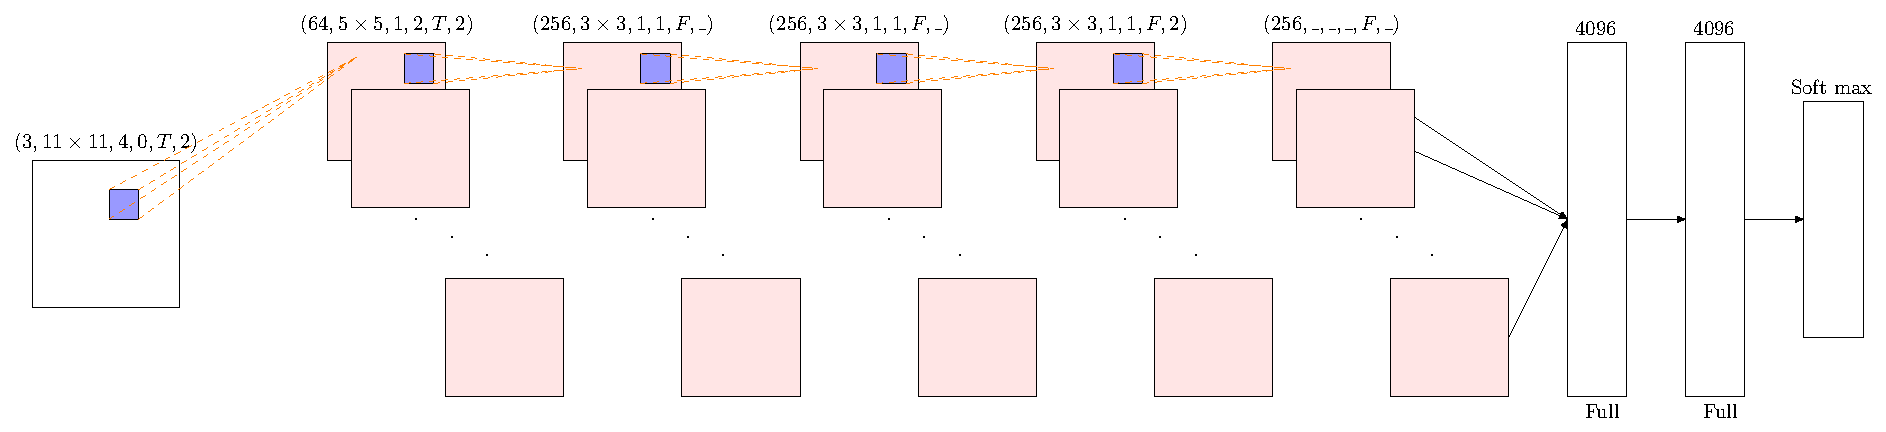
\includegraphics[scale=0.5]{./figures/nw.pdf}
  \caption{CNN architecture used for generating static features. The CNN consists of five convolution layers,
  two fully connected layers, and one softmax layer. The details of each convolutional layer are provided on top of each layer
  according to the following format:(number of convolution layers $\times$ filter width $\times$ filter height, convolution stride,
  spatial padding, is Local Response Normalization added, max-pooling factor). Value above fully connected layers indicates the dimensionality of the layer.
  We use \hl{ReLu} as the activation function.}
\label{fi:cnn}
\end{figure*} 